% Standalone source for the paper figure; build with figures/build.sh
\documentclass[border=1pt]{standalone}
% Shared preamble for the standalone figure sources.
\usepackage{times}
\usepackage{amsmath,amssymb}
\usepackage{xcolor}
\usepackage{textcomp}
\usepackage{tikz}
\usepackage{pgfplots}
\usetikzlibrary{arrows.meta,positioning,calc,fit,backgrounds}
\usepgfplotslibrary{fillbetween}
\pgfplotsset{compat=1.16}

% Colours are colour-blind safe (Okabe--Ito) and every figure also separates
% its classes by line style or fill, so the figures stay readable in greyscale.
\definecolor{cObs}{HTML}{0072B2}   % observed by the network
\definecolor{cHid}{HTML}{D55E00}   % hidden / unexplained
\definecolor{cHelp}{HTML}{009E73}  % safety helpers
\definecolor{cInk}{HTML}{333333}

\tikzset{
  box/.style={draw=cInk!70, rounded corners=1.5pt, fill=white, align=center,
              font=\scriptsize, inner sep=3pt, minimum height=0.8cm,
              line width=0.5pt},
  obs/.style={box, draw=cObs, fill=cObs!8},
  hid/.style={box, draw=cHid, fill=cHid!10},
  help/.style={box, draw=cHelp, fill=cHelp!10},
  flow/.style={-{Stealth[length=4pt]}, line width=0.6pt, draw=cInk!80},
  lbl/.style={font=\scriptsize, text=cInk!85, inner sep=1.5pt, align=center},
}
\pgfplotsset{
  every axis/.append style={font=\scriptsize, tick label style={font=\scriptsize},
                            label style={font=\scriptsize},
                            title style={font=\scriptsize\bfseries}, line width=0.5pt},
}

\begin{document}
\begin{minipage}[t]{5.64cm}
\centering
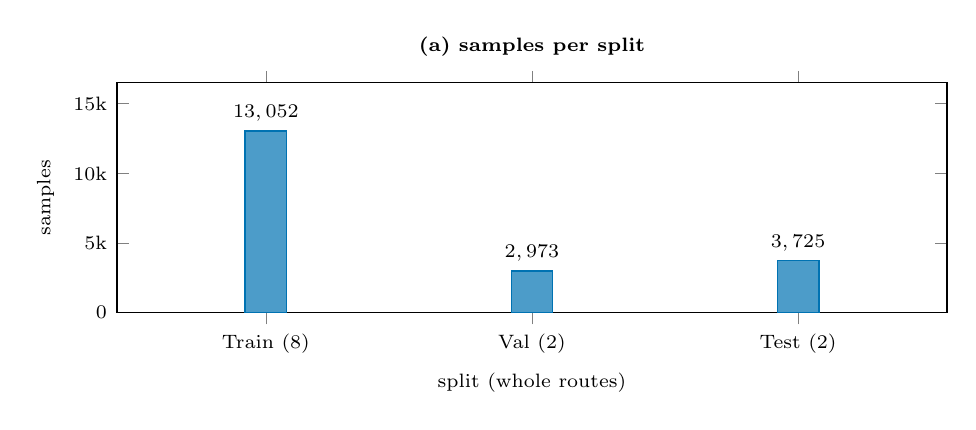
\begin{tikzpicture}[baseline=(current bounding box.north)]
\begin{axis}[ybar, width=\linewidth, height=4.5cm, bar width=15pt,
  symbolic x coords={Train,Val,Test}, xtick=data,
  xticklabels={Train (8),Val (2),Test (2)},
  ymin=0, ymax=16500, enlarge x limits=0.28,
  xlabel={split (whole routes)},
  ylabel={samples}, ytick={0,5000,10000,15000},
  yticklabels={0,5k,10k,15k}, scaled y ticks=false,
  title={(a) samples per split},
  nodes near coords, nodes near coords align={vertical},
  every node near coord/.append style={font=\scriptsize,
    /pgf/number format/fixed, /pgf/number format/precision=0,
    /pgf/number format/1000 sep={{,}}}]
  \addplot[fill=cObs!70, draw=cObs] coordinates {(Train,13052)(Val,2973)(Test,3725)};
\end{axis}
\end{tikzpicture}
\end{minipage}\hspace{0.635cm}
\begin{minipage}[t]{5.64cm}
\centering
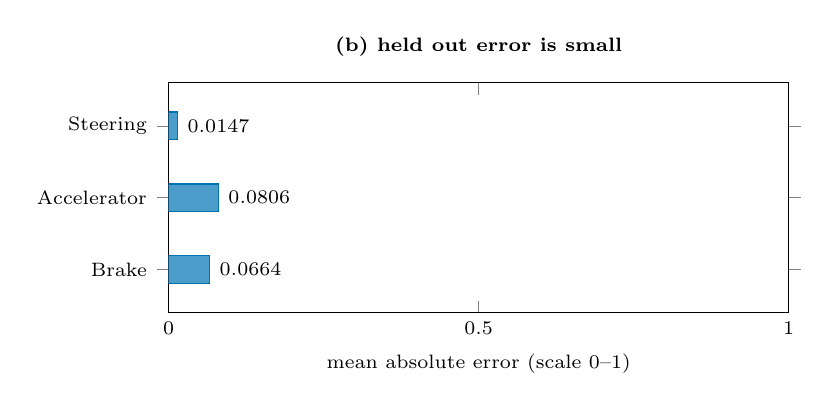
\begin{tikzpicture}[baseline=(current bounding box.north)]
\begin{axis}[xbar, width=0.78\linewidth, height=4.5cm, bar width=10pt,
  symbolic y coords={Brake,Accelerator,Steering}, ytick=data,
  xmin=0, xmax=1, enlarge y limits=0.3,
  xlabel={mean absolute error (scale 0--1)},
  xtick={0,0.5,1},
  title={(b) held out error is small},
  nodes near coords, nodes near coords align={horizontal},
  every node near coord/.append style={font=\scriptsize,
    /pgf/number format/fixed, /pgf/number format/precision=4}]
  \addplot[fill=cObs!70, draw=cObs] coordinates {(0.0664,Brake)(0.0806,Accelerator)(0.0147,Steering)};
\end{axis}
\end{tikzpicture}
\end{minipage}\hspace{0.635cm}
\begin{minipage}[t]{5.64cm}
\centering
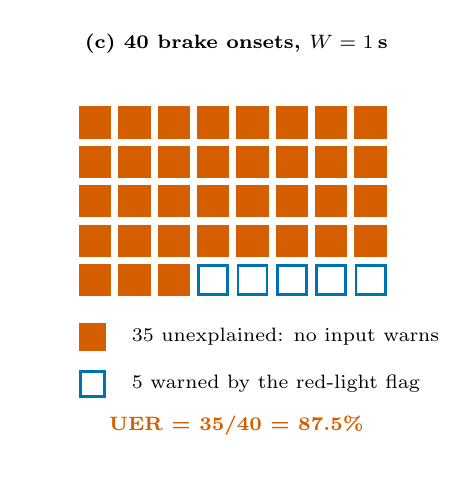
\begin{tikzpicture}[x=0.5cm,y=0.5cm,baseline=(current bounding box.north)]
\useasboundingbox (-1.3,-8.7) rectangle (9.3,2.0);
\node[font=\scriptsize\bfseries] at (4,1.6) {(c) 40 brake onsets, $W=1$\,s};
\foreach \i in {0,...,39}{
  \pgfmathtruncatemacro{\r}{int(\i/8)}
  \pgfmathtruncatemacro{\c}{mod(\i,8)}
  \ifnum\i<35
    \fill[cHid] (\c,-\r) rectangle ++(0.82,-0.82);
  \else
    \draw[cObs, fill=white, line width=1pt] (\c+0.04,-\r-0.04) rectangle ++(0.74,-0.74);
  \fi
}
\fill[cHid] (0,-5.5) rectangle ++(0.7,-0.7);
\node[font=\scriptsize, anchor=west] at (1.1,-5.85) {35 unexplained: no input warns};
\draw[cObs, fill=white, line width=1pt] (0.04,-6.74) rectangle ++(0.62,-0.62);
\node[font=\scriptsize, anchor=west] at (1.1,-7.05) {5 warned by the red-light flag};
\node[font=\scriptsize\bfseries, text=cHid] at (4,-8.1) {UER = 35/40 = 87.5\%};
\end{tikzpicture}
\end{minipage}
\end{document}
